\section{Contour Plots for the Calculated Significance with a Flat Uncertainty}\label{sec:Contours}
\begin{figure}[H]
    \vspace{-0.5cm}
    \makebox[0.95\linewidth][c]{%
    \centering
    \begin{subfigure}{.45\textwidth}
        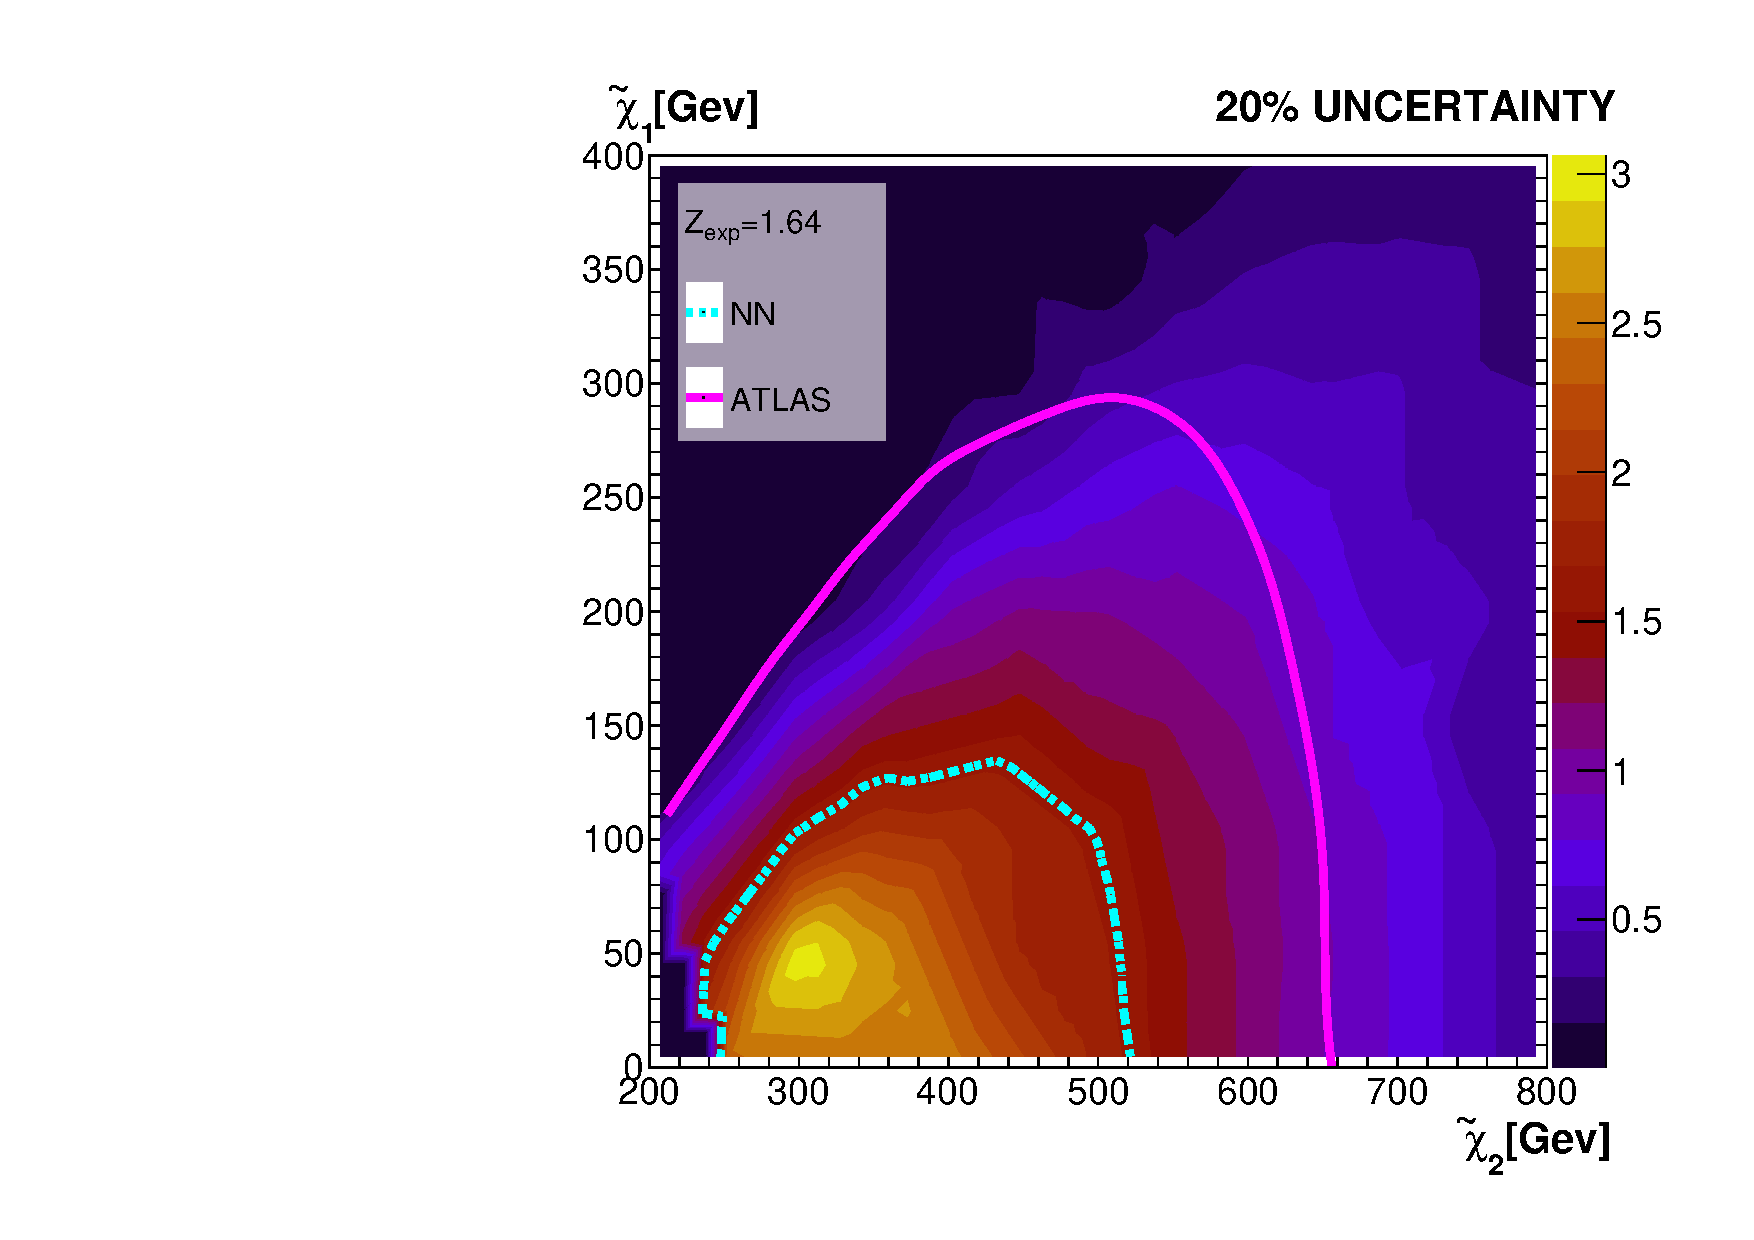
\includegraphics[width=\textwidth]{Figures/MLResults/NN/SUSY/Comparison/Limits/NNLimit20.pdf}
        \vspace{-0.75cm}
        \vspace*{-33.1ex}  % Tune this to the image height.
        \begin{center}
        \tiny
        \hspace{-44.5ex}
        \cite{atlas_search_2021}
        \end{center}
        \vspace*{34.1ex}
        \vspace{-1.cm}
        \caption{}
        \label{fig:NNLimit20}
    \end{subfigure}
    \hfill
    \begin{subfigure}{.45\textwidth}
        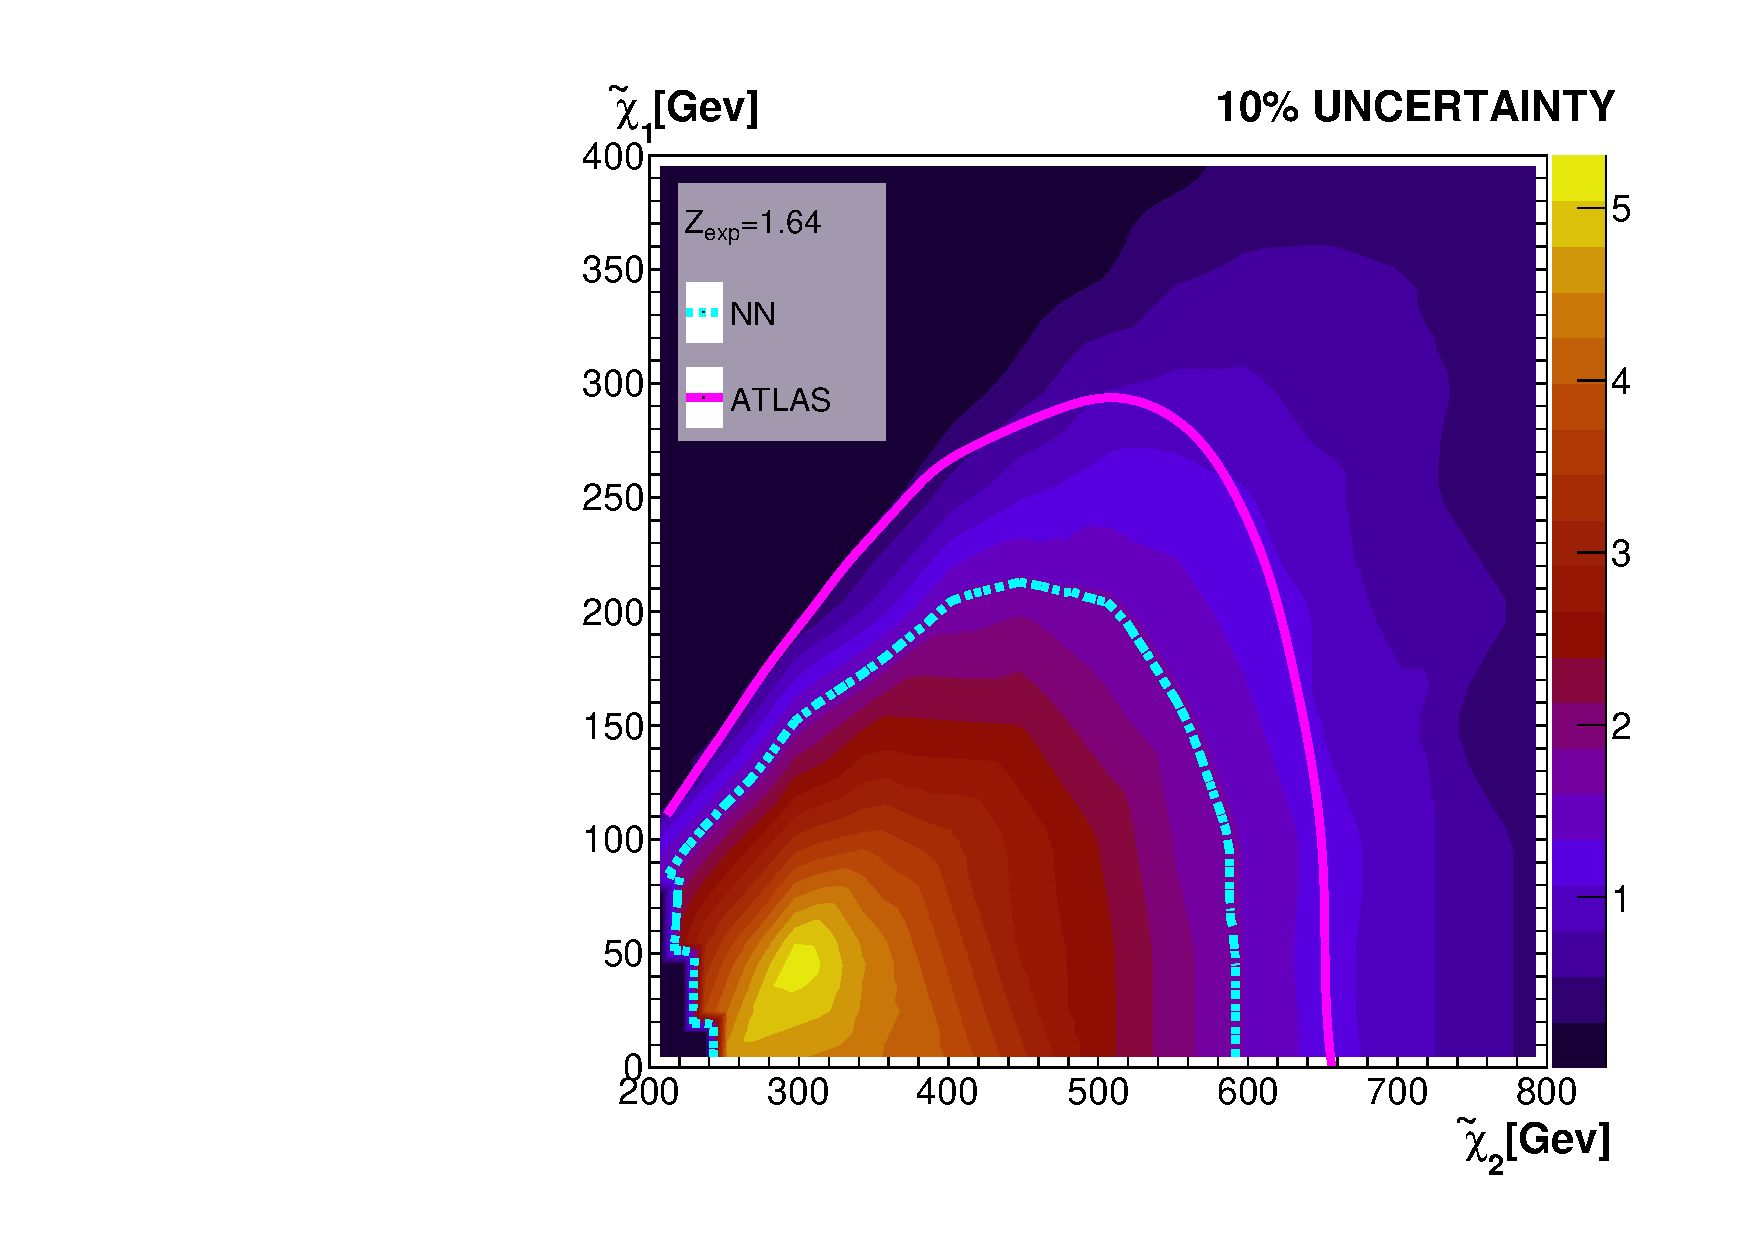
\includegraphics[width=\textwidth]{Figures/MLResults/NN/SUSY/Comparison/Limits/NNLimit10.pdf}
        \vspace{-0.75cm}
        \vspace*{-33.1ex}  % Tune this to the image height.
        \begin{center}
        \tiny
        \hspace{-44.5ex}
        \cite{atlas_search_2021}
        \end{center}
        \vspace*{34.1ex}
        \vspace{-1.cm}
        \caption{}
        \label{fig:NNLimit10}
    \end{subfigure}
    }
    \makebox[0.95\linewidth][c]{%
    \begin{subfigure}{.45\textwidth}
        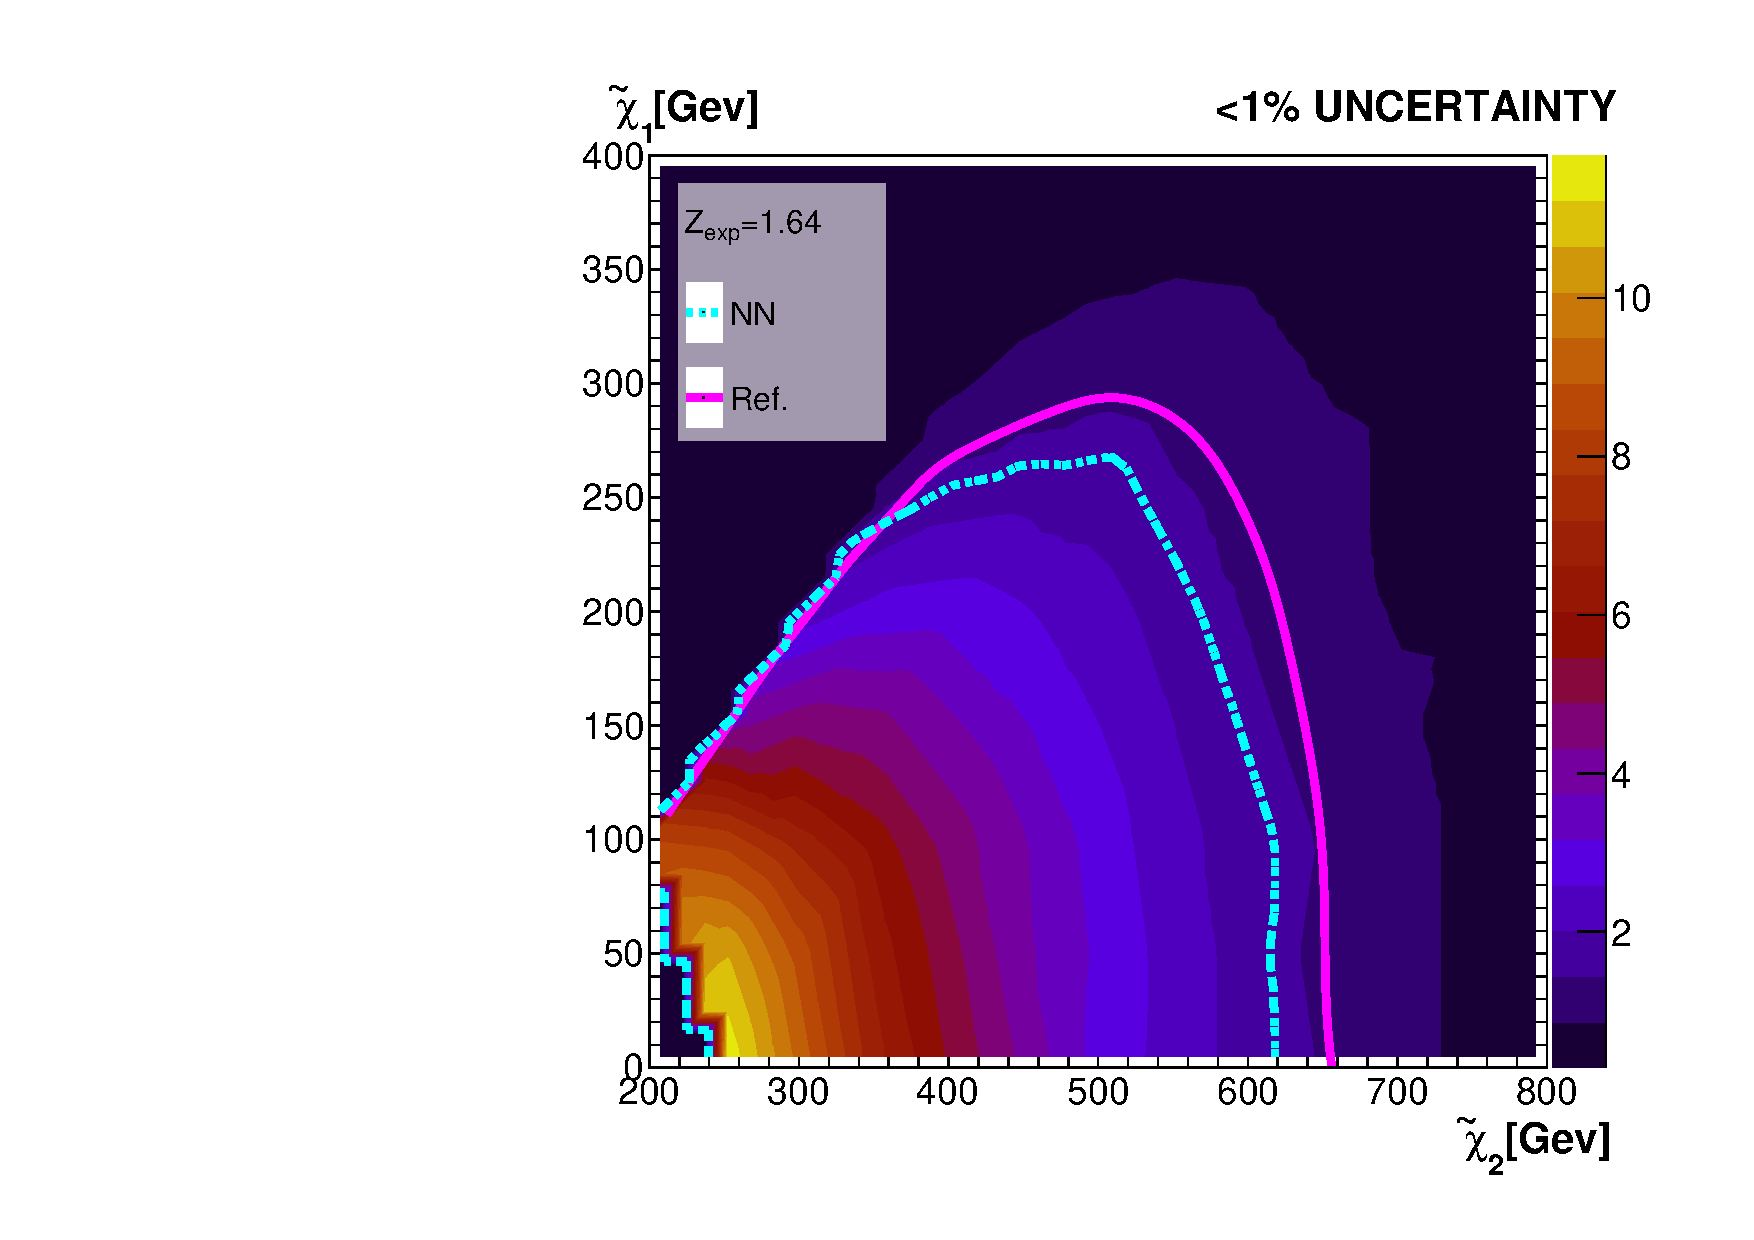
\includegraphics[width=\textwidth]{Figures/MLResults/NN/SUSY/Comparison/Limits/NNLimit1.pdf}
        \vspace{-0.75cm}
        \vspace*{-33.1ex}  % Tune this to the image height.
        \begin{center}
        \tiny
        \hspace{-44.5ex}
        \cite{atlas_search_2021}
        \end{center}
        \vspace*{34.1ex}
        \vspace{-1.cm}
        \caption{}
        \label{fig:NNLimit1}
    \end{subfigure}
    \hfill
    \begin{subfigure}{.45\textwidth}
        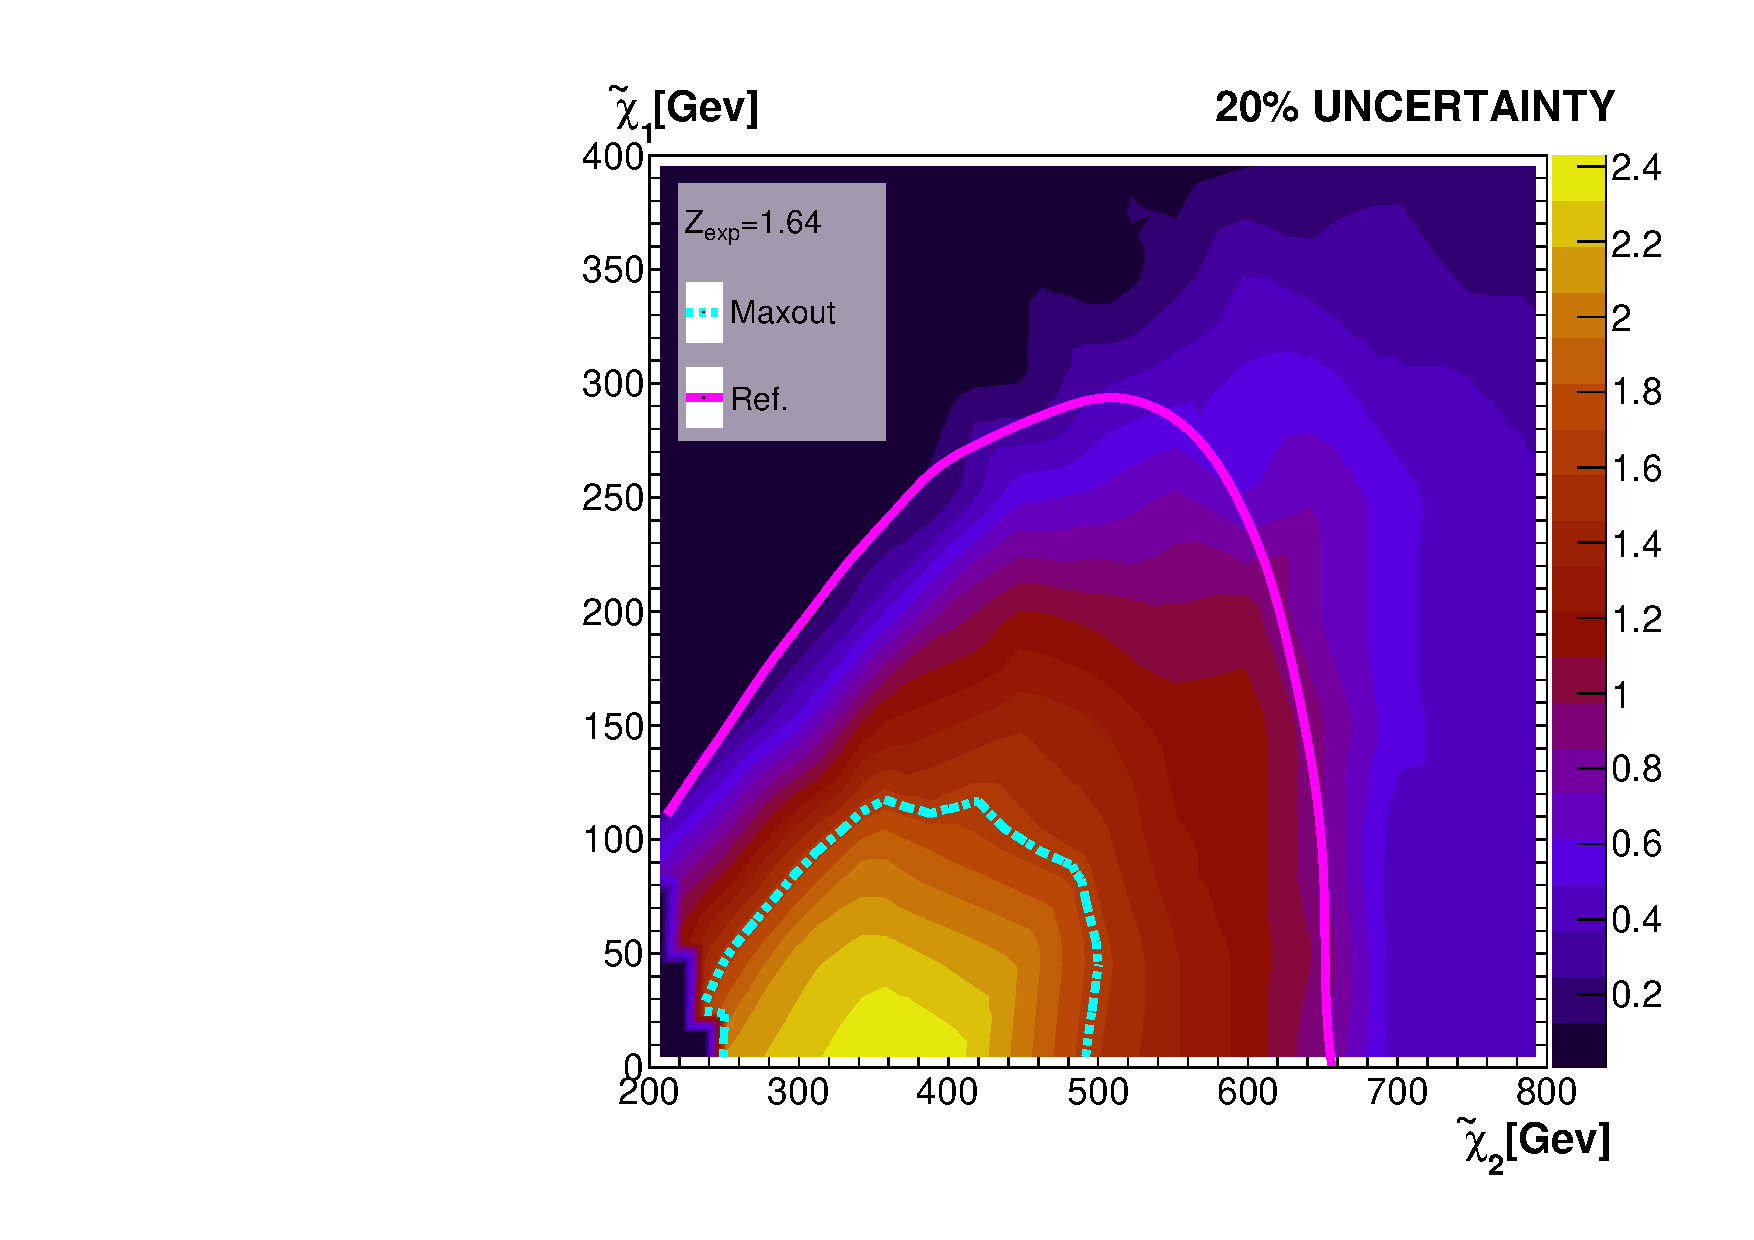
\includegraphics[width=\textwidth]{Figures/MLResults/NN/SUSY/Comparison/Limits/MaxOutLimit20.pdf}
        \vspace{-0.75cm}
        \vspace*{-33.1ex}  % Tune this to the image height.
        \begin{center}
        \tiny
        \hspace{-44.5ex}
        \cite{atlas_search_2021}
        \end{center}
        \vspace*{34.1ex}
        \vspace{-1.cm}
        \caption{}
        \label{fig:MaxOutLimit20}
    \end{subfigure}
    }
    \makebox[0.95\linewidth][c]{%
    \begin{subfigure}{.45\textwidth}
        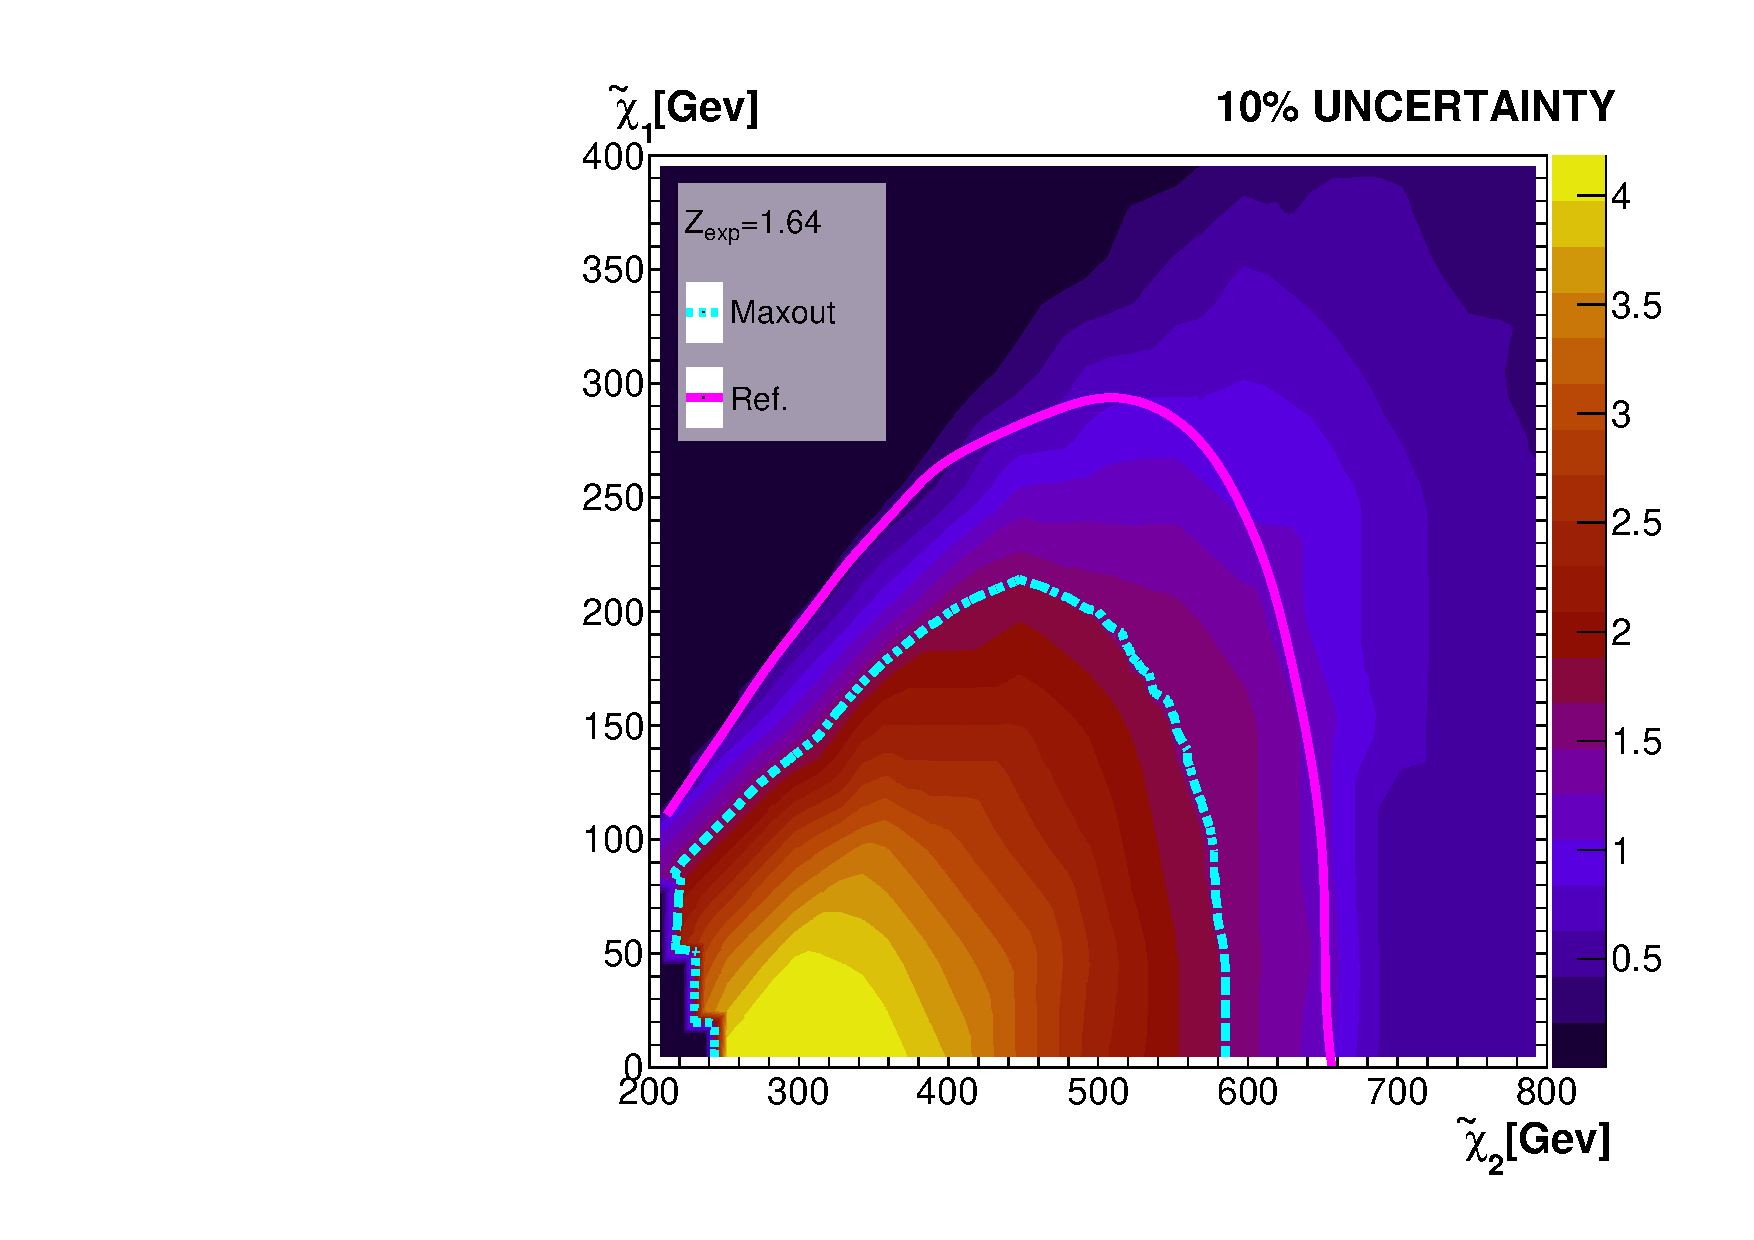
\includegraphics[width=\textwidth]{Figures/MLResults/NN/SUSY/Comparison/Limits/MaxOutLimit10.pdf}
        \vspace{-0.75cm}
        \vspace*{-33.1ex}  % Tune this to the image height.
        \begin{center}
        \tiny
        \hspace{-44.5ex}
        \cite{atlas_search_2021}
        \end{center}
        \vspace*{34.1ex}
        \vspace{-1.cm}
        \caption{}
        \label{fig:MaxOutLimit10}
    \end{subfigure}
    \hfill
    \begin{subfigure}{.45\textwidth}
        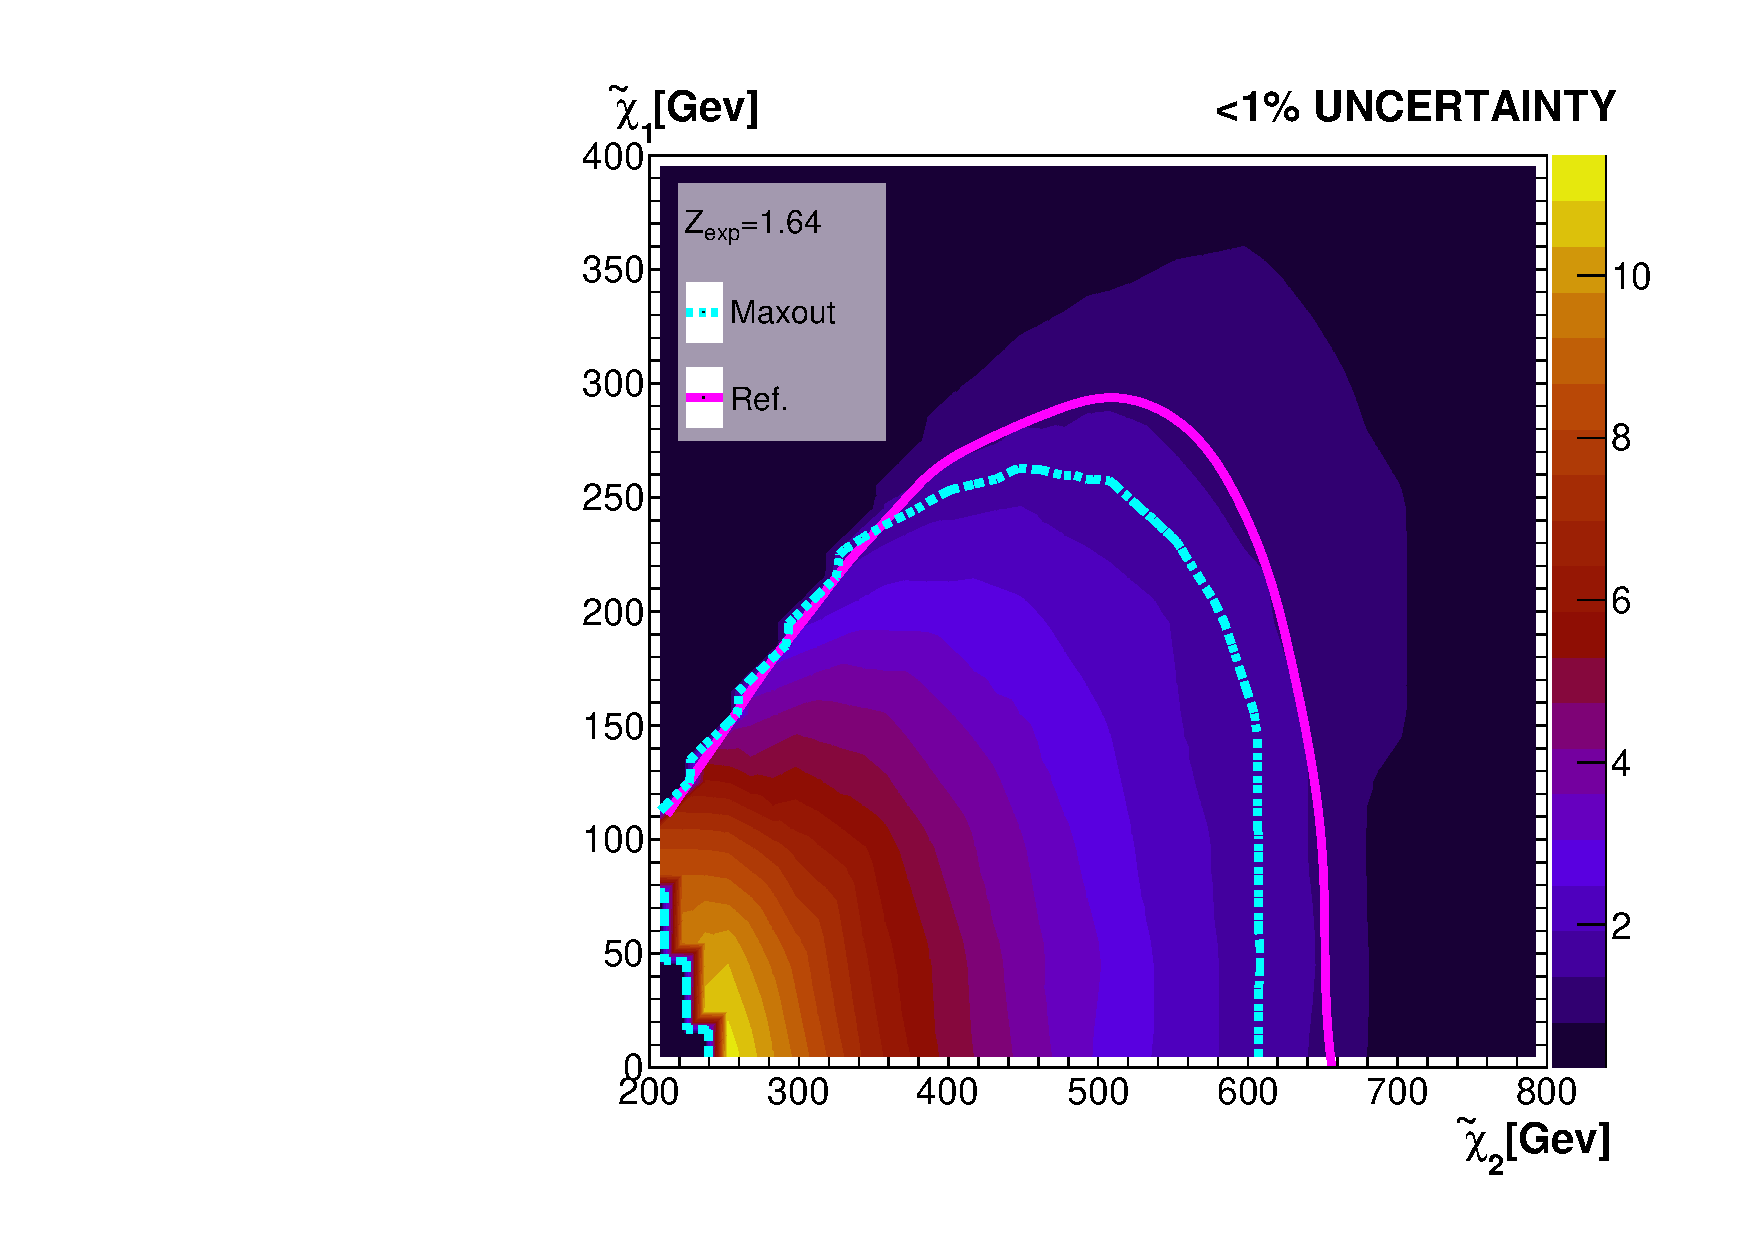
\includegraphics[width=\textwidth]{Figures/MLResults/NN/SUSY/Comparison/Limits/MaxOutLimit1.pdf}
        \vspace{-0.75cm}
        \vspace*{-33.1ex}  % Tune this to the image height.
        \begin{center}
        \tiny
        \hspace{-44.5ex}
        \cite{atlas_search_2021}
        \end{center}
        \vspace*{34.1ex}
        \vspace{-1.cm}
        \caption{}
        \label{fig:MaxOutLimit1}
    \end{subfigure}
    }
    \caption[Contour plots 
    of the significance achieved by the ordinary dense \acs{NN} and maxout model on the full statistics signal set. Contours are drawn 
    around the band equal to a significance of 1.64 for each model respectively (cyan) and for the \acs{ATLAS} analysis (pink).]{ Contour plots 
    of the significance achieved by the ordinary dense \acs{NN} and maxout model on the full statistics signal set. Contours are drawn 
    around the band equal to a significance of 1.64 for each model respectively (cyan) and for the \acs{ATLAS} analysis \cite{atlas_search_2021} (pink). The 
    significance achieved by the \acs{ML} models were calculated with a flat uncertainty equal to $20\%$ (\ref{fig:NNLimit20} and \ref{fig:MaxOutLimit20}),
    $10\%$ (\ref{fig:NNLimit10} and \ref{fig:MaxOutLimit10}) and $<1\%$ (\ref{fig:NNLimit1} and \ref{fig:MaxOutLimit1}) for the dense \acs{NN} and maxout model
    respectively.}
\end{figure}